Các miền phụ cốt lõi, hỗ trợ và chung có thể khác nhau đối với các doanh nghiệp hoạt động trong cùng một miền. Vì các miền phụ được xác định tùy theo nhu cầu kinh doanh và bối cảnh cụ thể của mỗi tổ chức.

\subsubsection{Mô tả cách xác định các miền phụ}

\begin{enumerate}

\item Bắt đầu bằng cách xem xét nghiệp vụ kinh doanh.

\item Nếu có sẵn giải pháp đã biết thì có khả năng là miền phụ chung. Ngược lại, chúng ta kiểm tra nghiệp vụ kinh doanh đó có thêm giá trị kinh doanh nào hay không?

\item Nếu không có giá trị kinh doanh thì chúng ta kiểm tra xem các miền phụ cốt lõi có phụ thuộc vào miền phụ này hay không? Nếu có thì có khả năng là miền phụ hỗ trợ. Nếu không thì đó là miền phụ chung.

\item Nếu miền phụ có tiềm năng bổ sung một số giá trị kinh doanh thì bước kiểm tra tiếp theo là xem liệu miền doanh nghiệp có độ phức tạp cao hay không?

\item Nếu miền doanh nghiệp không có độ phức tạp cao thì có khả năng là miền phụ hỗ trợ. Ngược lại thì nó có khả năng là miền phụ cốt lõi.

\end{enumerate}

\begin{figure}[h]

\centering

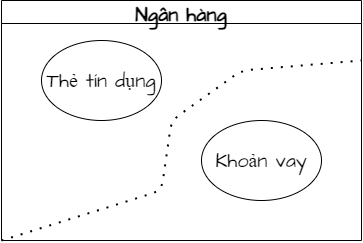
\includegraphics[scale = 0.5]{pictures/cach_xac_dinh_cac_mien_phu/main.drawio.png}

\caption{Sơ đồ xác định các miền phụ}

\end{figure}

